%================================================================
\chapter{Resultados}
%================================================================

\section{Testes}

\subsection{Ubuntu}
Para começar os testes no \textit{Ubuntu}, foi usada a versão 20.04 do mesmo onde primeiramente foi testado o pacote gerado através do empacotamento feito na \textit{Jaula-SID} que, como explicado anteriormente, cria um ambiente \textit{Debian Unstable} dentro do próprio \textit{Ubuntu}, gerando assim um pacote que contém dependências mais atualizadas do que as disponíveis no \textit{Ubuntu}. Este empacotamento segue as politicas do Debian e também se baseia parcialmente no \textbf{Manual de Empacotamento de Debian} que pode ser obtido em sua versão traduzida para o português através do endereço: \url{https://www.debian.org/doc/manuals/packaging-tutorial/packaging-tutorial.pt.pdf}.
 
Devido a esse problema de compatibilidade os primeiro testes acabaram gerando erro durante a instalação do pacote, e esses erros não eram contornáveis, uma vez que esses pacotes cujo o pacote E-foto tinha como dependência não tinham essas versões disponíveis de maneira alguma no \textit{Ubuntu 20.04}. 

Após algum tempo de estudo e pesquisas foi decidido o teste através da realização de um empacotamento diretamente no Ubuntu 20.04, sem a utilização da \textit{Jaula-SID} ou qualquer outro tipo de ambiente \textit{Debian Unstable}. Seguindo novamente de maneira parcial o \textbf{Manual de Empacotamento de Debian} e também o passo-a-passo que foi descrito aqui anteriormente, ocorreu a criação de um novo pacote com sucesso, porém durante a compilação do mesmo um novo erro \textit{lintian} apareceu, que trazia a mensagem retratando que o sistema operacional em que um novo pacote deve ser criado é o \textit{Debian Unstable} e que a versão do sistema operacional usado estava entrando em conflito com essa política.

Mas mesmo com essa nova mensagem de advertência, a compilação ocorreu com sucesso assim como a geração do pacote e após isso, foi só instalar o pacote através do comando:

\begin{lstlisting}[language=bash]
	$ sudo dpkg -i nome_do_pacote 
\end{lstlisting}

como pode ser visto na figura \ref{fig:ubuntu_insta}, buscar o caminho do diretório onde o \textit{E-foto} foi instalado através do terminal e utilizar o comando:

\begin{lstlisting}[language=bash]
	$ ./efoto
\end{lstlisting}

no diretório onde fica o executável, geralmente \textit{usr/bin} como é mostrado na figura \ref{fig:ubuntu_exec}.

\begin{figure}[!ht]{17cm}
	\centering
	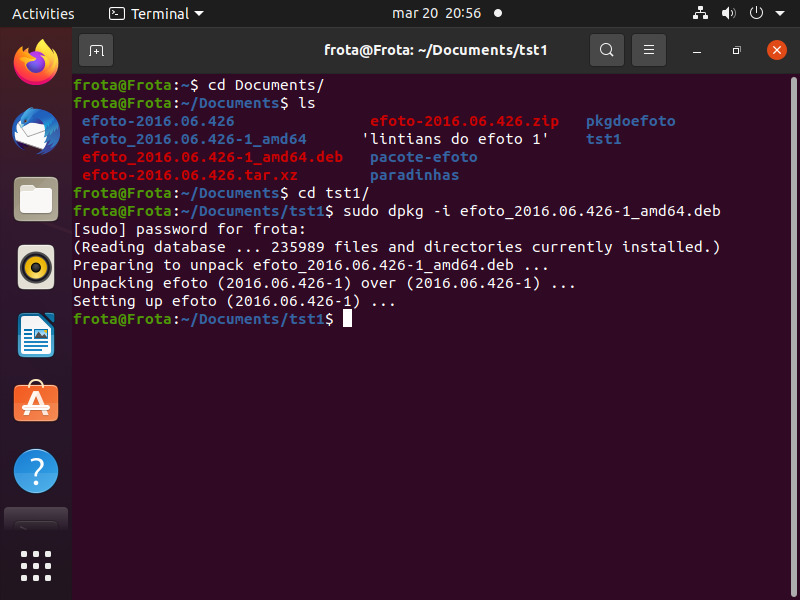
\includegraphics[width=15cm]{Figuras/ubuntu_insta.jpg}
	\caption{Instalação do pacote E-foto no Ubuntu} \label{fig:ubuntu_insta}
\end{figure}

\begin{figure}[!ht]{17cm}
	\centering
	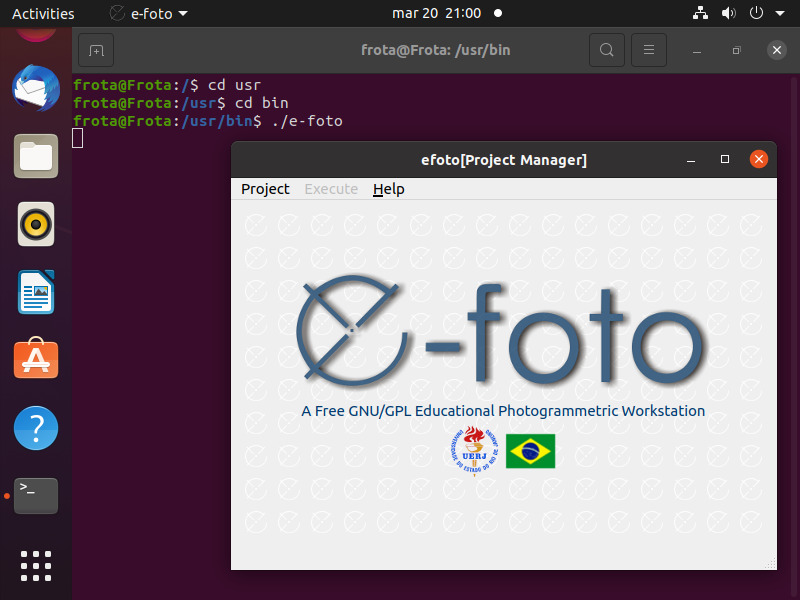
\includegraphics[width=15cm]{Figuras/ubuntu_exec.jpg}
	\caption{Funcionamento do executável gerado pelo pacote E-foto no Ubuntu} \label{fig:ubuntu_exec}
\end{figure}


\subsection{Debian Unstable}

Para começar o teste do funcionamento do pacote do software E-foto no sistema operacional \textit{Debian} em sua versão instável completa, que é o ambiente correto para a realização destes teste devido á ser neste ambiente que o próprio Debian realizará a primeira etapa de testes quando o pacote for finalizado e disponibilizado, é necessária a obtenção dessa versão instável do Debian, e para isso são necessários alguns passos, uma vez que essa versão não é disponibilizada diretamente para download no site do Debian. O método escolhido para instalação da versão instável do Debian foi através da alteração do arquivo \textbf{source.list} através do terminal de comando na versão do \textit{Debian testing} mais atual. 

O primeiro passo é a realização do download da versão mais atual do \textit{Debian testing} mais atual, que pode ser obtida através do endereço \url{https://www.debian.org/devel/debian-installer} e que poderá ser instalada em uma máquina própria ou em uma máquina virtual. Após a instalação do sistema operacional \textit{Debian Testing}, a próxima etapa é a edição do arquivo \textbf{source.list} através da linha de comando no caminho \textit{/etc/apt/source.list} substituindo o seu conteúdo com pelo seguinte:

\begin{verbatim}
deb http://ftp.br.debian.org/debian/ unstable main contrib non-free	
deb-src http://ftp.br.debian.org/debian/ unstable main contrib non-free
\end{verbatim}

Depois é preciso salvar e sair. Novamente no terminal de comando deve ser usado o comando:

\begin{lstlisting}[language=bash]
	$ sudo apt update
\end{lstlisting}

para que todos as listas de pacotes possam ser atualizadas, obtendo assim as versões mais recentes de cada pacote disponível no local especificado pelo \textbf{source.list} e depois o ultimo passo é o comando:

\begin{lstlisting}[language=bash]
	$ sudo apt upgrade
\end{lstlisting}

que instalará as versões mais recentes de todos os pacotes que já estão instalados no sistema baseados no local especificado pelo arquivo \textbf{source.list}. Com o fim da realização destes passos, a versão instável do Debian estará disponível para uso e consequentemente para a realização do teste do pacote.

Para testar o funcionamento do pacote, é preciso ir através do terminal de comando até o local onde está o arquivo .deb do E-foto e utilizar o comando:

\begin{lstlisting}[language=bash]
	$ sudo dpkg -i nome_do_pacote
\end{lstlisting}

que a instalação ocorrerá automaticamente como é demonstrado na figura \ref{fig:debian_insta}, porém para que isso aconteça o pacote \textbf{libgdal.dev} deve estar instalado previamente, após a instalação ser concluída, basta ir até o local onde foi instalado o E-foto, buscar o seu arquivo executável, que geralmente é instalado no \textit{usr/bin}, e usar o comando:

\begin{lstlisting}[language=bash]
	$ ./efoto
\end{lstlisting}

que o programa será executado perfeitamente como pode ser visto na figura \ref{fig:debian_exec}.

\begin{figure}[!ht]{17cm}
	\centering
	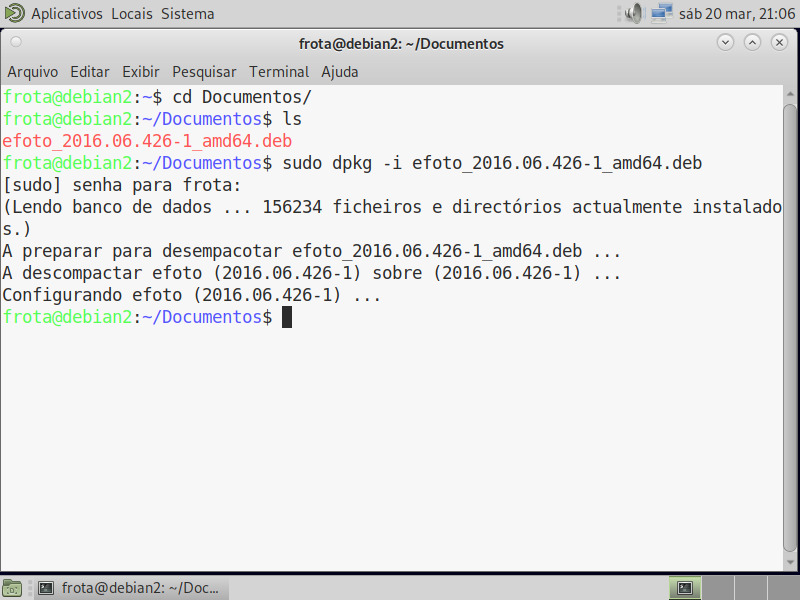
\includegraphics[width=15cm]{Figuras/debian_insta.jpg}
	\caption{Instalação do pacote E-foto no Debian} \label{fig:debian_insta}
\end{figure}

\begin{figure}[!ht]{17cm}
	\centering
	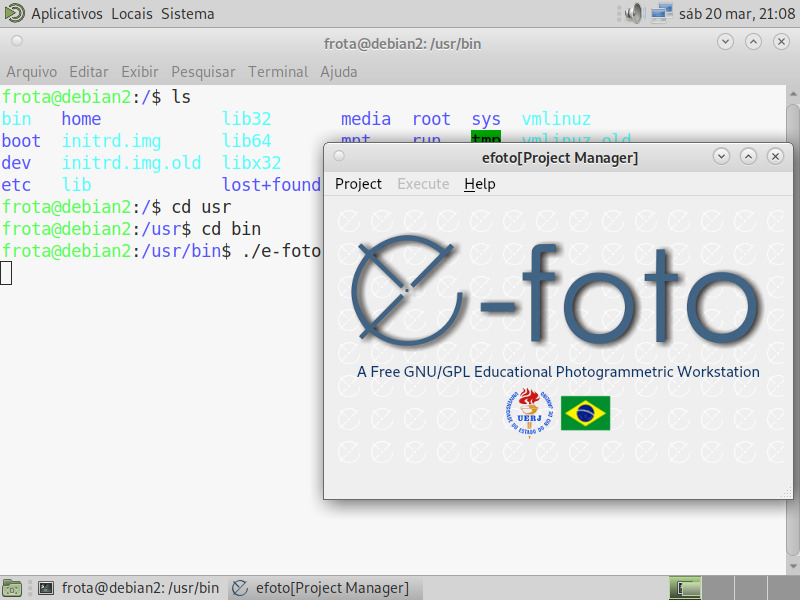
\includegraphics[width=15cm]{Figuras/debian_exec.jpg}
	\caption{Funcionamento do executável gerado pelo pacote E-foto no Debian} \label{fig:debian_exec}
\end{figure}